% !TeX root = ..\studio-operation-guide.tex
\section{Placing Calls}
You can place a call in one of three ways using your SIP-T28P IP phone:

\begin{itemize}
	\item Using the handset
	\item Using the speakerphone
	\item Using the headset
\end{itemize}

You can also dial the number first, and then choose the way you want to
speak to the other party.

You can also search and dial a contact from call history, local
directory or remote phone book. For more information, refer to Contact
Management on page 31 and Call History Management on page 48.

During a call, you can alternate between Speakerphone, Headset, and
Handset modes by pressing the Speakerphone key, the HEADSET key, or by
picking up the handset.

The call duration of the active call is visible on the LCD screen. In
the figure below, the call to the number''1005'' has lasted 6 seconds.

\begin{figure}[h]
	\centering
	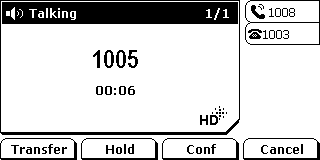
\includegraphics{images/yealink/screen-001.png}
\end{figure}

\subsubsection{To place a call using the handset:}

\begin{enumerate}
	\item Pick up the handset.
	\item Enter the desired number using the keypad.
	\item Press \scalerel*{
\includegraphics{images/yealink/btn-ok.png}}{B},
		\scalerel*{
\includegraphics{images/yealink/btn-hash.png}}{B}, or the
		\textbf{Send} soft key.
\end{enumerate}

The \# key is configured as a send key by default. You can also set the
* key as the send key, or set neither. For more information, refer to
Key as Send on page 24.

\begin{quote}
	\textbf{Note}
	
	You can also dial using the SIP URI or IP address. To obtain the IP
	address of the phone, press the OK key when the phone is idle. The
	maximum SIP URI or IP address length is 32 characters. For example, SIP
	URI: 2210@sip.com, IP: 192.168.1.15.

	Your phone may not support direct IP dialing. Contact your system
	administrator for more information.
\end{quote}

\subsubsection{To place a call using the hands-free speakerphone mode:}

Do one of the following:

\begin{itemize}
	\item With the handset on-hook, press
		\scalerel*{
\includegraphics{images/yealink/btn-speaker.png}}{B}
		or the line key to obtain a dial tone.

		Enter the desired number using the keypad.

		Press \scalerel*{
\includegraphics{images/yealink/btn-ok.png}}{B},
		\scalerel*{
\includegraphics{images/yealink/btn-hash.png}}{B}, or the
		\textbf{Send} soft key.
	\item With the handset on-hook, enter the desired number using the keypad.

		Press \scalerel*{
\includegraphics{images/yealink/btn-ok.png}}{B},
		\scalerel*{
\includegraphics{images/yealink/btn-hash.png}}{B}, or the
		\textbf{Send} soft key.
\end{itemize}

\subsubsection{To place a call using the headset:}

Do one of the following:

\begin{itemize}
	\item With the optional headset connected, press
		\scalerel*{
\includegraphics{images/yealink/btn-headset.png}}{B}
		to activate the headset mode.

		Press the line key to obtain a dial tone.

		Enter the desired number using the keypad.

		Press \scalerel*{
\includegraphics{images/yealink/btn-ok.png}}{B},
		\scalerel*{
\includegraphics{images/yealink/btn-hash.png}}{B}, or the
		\textbf{Send} soft key.
	\item With the optional headset connected, press
		\scalerel*{
\includegraphics{images/yealink/btn-headset.png}}{B}
		to activate the headset mode.

		Enter the desired number using the keypad.

		Press \scalerel*{
\includegraphics{images/yealink/btn-ok.png}}{B},
		\scalerel*{
\includegraphics{images/yealink/btn-hash.png}}{B}, or the
		\textbf{Send} soft key.
\end{itemize}

\begin{quote}
	\textbf{Note}
	
	To permanently activate the headset mode, refer to Headset Prior on page 51.
\end{quote}

The SIP-T28P IP phone can handle multiple calls at a time. However, only one
active call (the call that has audio associated with it) can be in progress at
any given time. The SIP-T28P IP phone can handle a maximum of 6 calls at one
time.

\subsubsection{To place multiple calls:}

You can have more than one call on your SIP-T28P IP phone. To place a
new call during an active call, do one of the following:

\begin{itemize}
	\item Press the line key. The active call is placed on hold.
		Enter the desired number using the keypad.

		Press \scalerel*{
\includegraphics{images/yealink/btn-ok.png}}{B},
		\scalerel*{
\includegraphics{images/yealink/btn-hash.png}}{B}, or the
		\textbf{Send} soft key.
	\item Press \scalerel*{
\includegraphics{images/yealink/btn-hold.png}}{B}
		or the \textbf{Hold} soft key to place the original call on hold.

		Press the \textbf{New Call} soft key.

		Enter the desired number using the keypad.

		Press \scalerel*{
\includegraphics{images/yealink/btn-ok.png}}{B},
		\scalerel*{
\includegraphics{images/yealink/btn-hash.png}}{B}, or the
		\textbf{Send} soft key.
\end{itemize}

You can press \scalerel*{
\includegraphics{images/yealink/btn-up.png}}{B} or
\scalerel*{
\includegraphics{images/yealink/btn-down.png}}{B} to switch between
the calls, and then press the \textbf{Resume} soft key to retrieve the desired
call.

\begin{quote}
	\textbf{Note}
	
	If multiple accounts are registered on the phone, you can first press
	the desired line key in the idle screen or press the Line soft key in
	the dialing screen, and then you can use the selected account to place a
	call.
\end{quote}
